\section{Experiments}

Results on our validation sets are shown in Figure~\ref{fig:quant}. We first evaluate how well our metrics and networks work. All validation sets contain 5 pairwise judgments for each triplet. Because this is an inherently noisy process, we compute agreement of an algorithm with \textit{all} of the judgments. For example, if there are 4 preferences for $x_0$ and 1 for $x_1$, an algorithm which predicts the more popular choice $x_0$ would receive $80\%$ credit. If a given example is scored with fraction $p$ humans in one direction and $1-p$ in the other, a human would achieve score $p^2+(1-p)^2$ on expectation.

\subsection{Evaluations}

\begin{figure}[t]
  \centering
  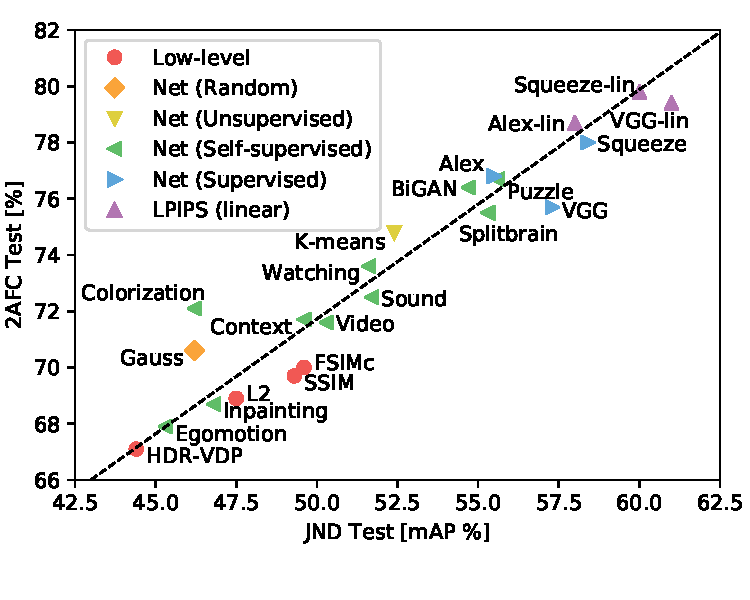
\includegraphics[width=1.\linewidth]{imgs/trip_vs_jnd.pdf}
\vspace{-12mm}
\caption{\textbf{Correlating Perceptual Tests.} We show performance across methods, including unsupervised~\cite{krahenbuhl2015data}, self-supervised~\cite{agrawal2015learning,pathakCVPR16context,doersch2015unsupervised,wang2015unsupervised,zhang2016colorful,owens2016visually,pathak2017learning,noroozi2016unsupervised,donahue2016adversarial,zhang2017split}, supervised~\cite{krizhevsky2014one,simonyan2014very,iandola2016squeezenet}, and our perceptually-learned metrics (LPIPS). The scores are on our 2AFC and JND tests, averaged across traditional and CNN-based distortions.}
\label{fig:trip_vs_jnd}
\vspace{-2mm}
\end{figure}

\paragraph{How well do low-level metrics and classification networks perform?} Figure~\ref{fig:quant} shows the performance of various low-level metrics (in red), deep networks, and human ceiling (in black). The scores are averaged across the 2 distortion test sets (traditional+CNN-based) in Figure~\ref{fig:quant} (left), and 4 real algorithm benchmarks (superresolution, frame interpolation, video deblurring, colorization) in Figure~\ref{fig:quant} (right). All scores within each test set are shown in the appendix. Averaged across all 6 test sets, humans are $73.9\%$ consistent. Interestingly, the supervised networks perform at about the same level to each other, at $68.6\%$, $68.9\%$, and $67.0\%$, even across variation in model sizes -- SqueezeNet ($2.8$ MB), AlexNet ($9.1$ MB), and VGG ($58.9$ MB) (only convolutional layers are counted). They all perform better than traditional metrics $\ell_2$, SSIM, and FSIM at $63.2\%$, $63.1\%$, $63.8\%$, respectively. Despite its common use, SSIM was not designed for situations where geometric distortion is a large factor~\cite{sampat2009complex}.

\paragraph{Does the network have to be trained on classification?} In Figure~\ref{fig:quant}, we show model performance across a variety of unsupervised and self-supervised tasks, shown in green -- generative modeling with BiGANs~\cite{donahue2016adversarial}, solving puzzles~\cite{noroozi2016unsupervised}, cross-channel prediction~\cite{zhang2017split}, and segmenting foreground objects from video~\cite{pathak2017learning}. These self-supervised tasks perform on par with classification networks. This indicates that tasks across a large spectrum can induce representations which transfer well to perceptual distances. Also, the performance of the stacked k-means method~\cite{krahenbuhl2015data}, shown in yellow, outperforms low-level metrics. Random networks, shown in orange, with weights drawn from a Gaussian, do not yield much improvement. This indicates that the combination of network structure, along with orienting filters in directions where data is more dense, can better correlate to perceptual judgments.

\subfile{tables/correlation}

In Table~\ref{fig:trip_vs_jnd}, we explore how well our perceptual task correlates to semantic tasks on the PASCAL dataset~\cite{pascal-voc-2007}, using results summarized in~\cite{zhang2017split}, including additional self-supervised methods~\cite{agrawal2015learning,pathakCVPR16context,doersch2015unsupervised,wang2015unsupervised,zhang2016colorful,owens2016visually}. We compute the correlation coefficient between each task (perceptual or semantic) across different methods. The correlation from our 2AFC distortion preference task to classification and detection is .640 and .363, respectively. Interestingly, this is similar to the correlation between the classification and detection tasks (.429), even though both are considered ``high-level" semantic tasks, and our perceptual task is ``low-level."

\begin{figure*}
\centering
\begin{subfigure}{1.\textwidth}
  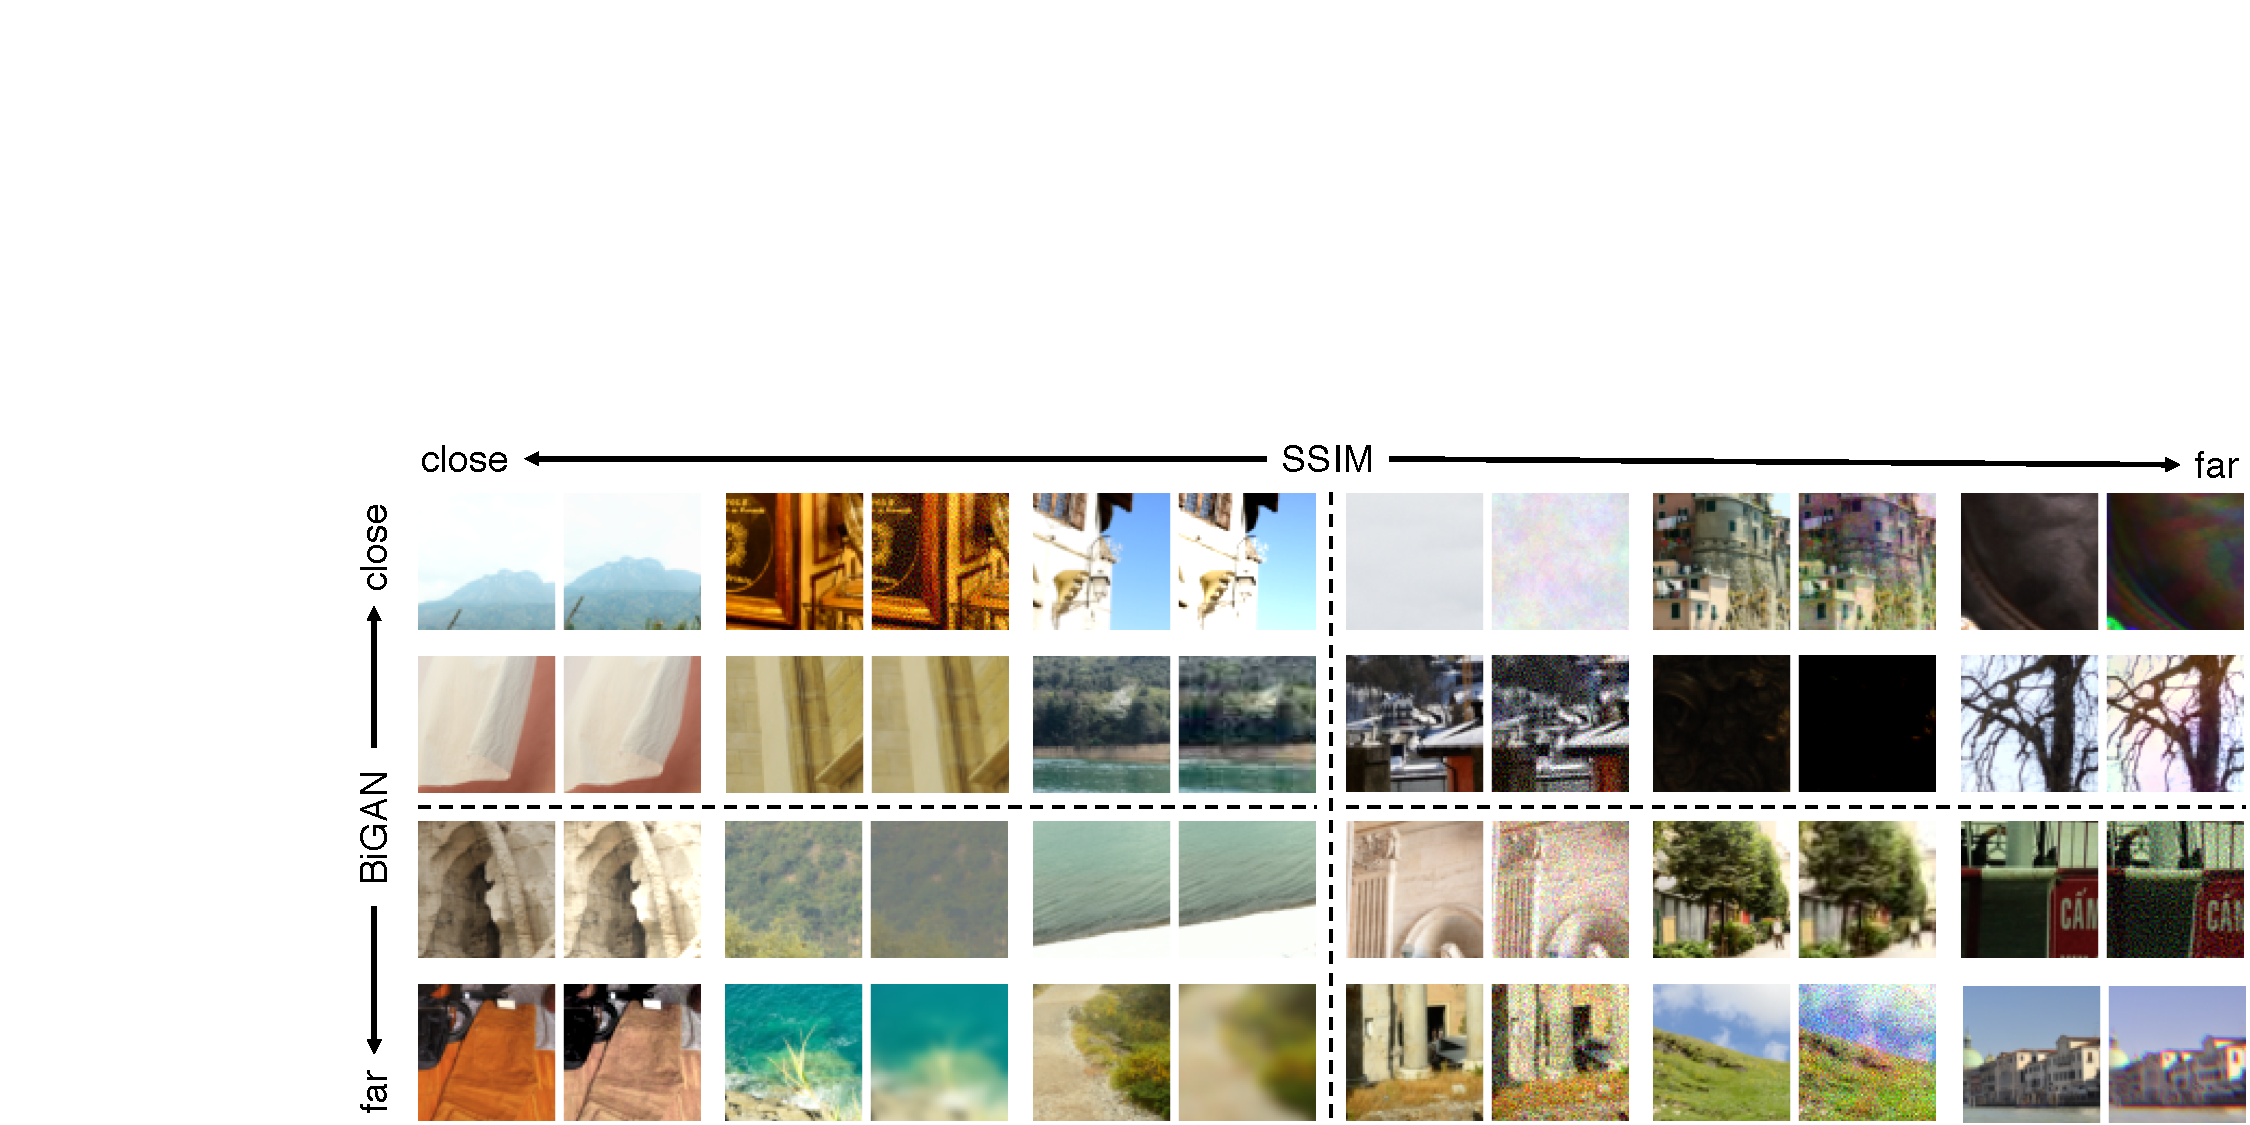
\includegraphics[width=1.\linewidth]{imgs/fig_comp_low.pdf}
  \vspace{-5mm}
\end{subfigure}
\caption{\textbf{Qualitative comparisons on distortions.} We show qualitative comparison on traditional distortions, using the SSIM~\cite{wang2004image} metric and BiGAN network~\cite{donahue2016adversarial}. We show examples where the metrics agree and disagree. A primary difference is that deep embeddings appear to be more sensitive to blur. Please see the appendix for additional examples.}
\label{fig:qual_comp}
\vspace{-4mm}
\end{figure*}

\paragraph{Do metrics correlate across different perceptual tasks?} We test if training for the 2AFC distortion preference test corresponds with another perceptual task, the JND test. We order patch pairs by ascending order by a given metric, and compute precision-recall on our CNN-based distortions -- for a good metric, patches which are close together are more likely to be confused for being the same. We compute area under the curve, known as mAP~\cite{pascal-voc-2007}. The 2AFC distortion preference test has high correlation to JND: $\rho=.928$ when averaging the results across distortion types. Figure~\ref{fig:trip_vs_jnd} shows how different methods perform under each perceptual test. This indicates that 2AFC generalizes to another perceptual test and is giving us signal regarding human judgments.

\paragraph{Can we train a metric on traditional and CNN-based distortions?} In Figure~\ref{fig:quant}, we show performance using our \tbfit{lin}, \tbfit{scratch}, and \tbfit{tune} configurations, shown in purple, pink, and brown, respectively. When validating on the traditional and CNN-based distortions (Figure~\ref{fig:quant}(a)), we see improvements. Allowing the network to tune all the way through (brown) achieves higher performance than simply learning linear weights (purple) or training from scratch (pink). The higher capacity network VGG also performs better than the lower capacity SqueezeNet and AlexNet architectures. These results verify that networks can indeed learn from perceptual judgments.

\paragraph{Does training on traditional and CNN-based distortions transfer to real-world scenarios?} We are more interested in how performance generalizes to \textit{real-world algorithms}, shown in Figure~\ref{fig:quant}(b). The SqueezeNet, AlexNet, and VGG architectures start at $64.0\%$, $65.0\%$, and $62.6\%$, respectively. Learning a linear classifier (purple) improves performance for all networks. Across the 3 networks and 4 real-algorithm tasks, 11 of the 12 scores improved, indicating that ``calibrating" activations on a pre-existing representation using our data is a safe way to achieve a small boost in performance ($1.1\%$, $0.3\%$, and $1.5\%$, respectively). Training a network from scratch (pink) yields slightly lower performance for AlexNet, and slightly higher performance for VGG than linear calibration. However, these still outperform low-level metrics. This indicates that the distortions we have expressed do project onto our test-time tasks of judging real algorithms. 

Interestingly, starting with a pre-trained network and tuning throughout \textit{lowers} transfer performance. This is an interesting negative result, as training for a low-level perceptual task directly does not necessarily perform as well as transferring a representation trained for the high-level task.

\paragraph{Where do deep metrics and low-level metrics disagree?} In Figure~\ref{fig:qual_comp}, we show a qualitative comparison across our traditional distortions for a deep method, BiGANs~\cite{donahue2016adversarial}, and a representation traditional perceptual method, SSIM~\cite{wang2004image}. Pairs which BiGAN perceives to be far but SSIM to be close generally contain some blur. BiGAN tends to perceive correlated noise patterns to be a smaller distortion than SSIM.
